% !TeX encoding = UTF-8
% !TeX spellcheck = en_US
% !TeX root = ../MasterThesis_OlivierChurlaud_2016.tex

\chapter{Introduction}
\label{sec:background}

\section{BESSY II -- General presentation}
BESSY II (\textbf{B}erliner \textbf{E}lektronen\-\textbf{S}peicherring-Gesellschaft für \textbf{Sy}n\-chro\-tron\-strahlung m.b.H.) is Berlin electron storage ring, aimed at producing high energy light ray by synchrotron radiation. It emits extremely brilliant photons pulse ranging from the long wave terahertz region to hard X rays, with an emphasis on the soft X-ray range\todo{figure spectrum}~\cite{web:bessy_homepage}.

Scientific projects can freely apply to an experimental station, where they are able to adjust the wavelength, polarization and photon energy. More than 2000 scientists per year are using BESSY II equipment.

The storage ring has a circumference of \SI{240}{\meter} and provides around 50 beamlines (paths of light rays between the accelerator and experimental stations). The electrons are accelerated to an energy up to \SI{1.7}{\giga\electronvolt}.

BESSY II was inaugurated in 1998 and is since 2009 a facility of the \textit{Helmholtz-Zentrum Berlin für Materialien und Energie} (HZB), to study material structures and processes by guest scientists.

Additionally to the guest scientists, operators and researchers ensure the good functioning of the whole facility and work on refining the quality and the stability of the light rays.

\section{BESSY II -- General functioning}
In BESSY II  accelerator, particle are circularly accelerated, all of them turning in the same direction. The goal is indeed not to produce collisions but light.

The way BESSY II functions is based on the synchrotron radiation phenomenon: any accelerated particle emits radiations (in the form of photons), with a maximal amplitude in the case of a circular acceleration. It can be shown~\cite{book:wille} that the radiated power in circular acceleration can be given as
\begin{equation}
P_s = \frac{e^2 c}{6 \pi \varepsilon_0}\frac{1}{(m_0 c^2)^4}\frac{E^4}{R^2}.
\end{equation}
where $c$ is the speed of light, $m_0$ the rest mass (independent of the velocity) of the particle, $e$ its charge, $E$ its energy, $R$ the bending radius and $\varepsilon_0$ the  vacuum permittivity.

Considering their low mass, the electrons are very good candidates to produce high energy radiation (in comparison, accelerated protons would provide a power $10^{13}$ smaller than electrons), and are therefore used in BESSY~II.

\begin{figure}
    \centering
    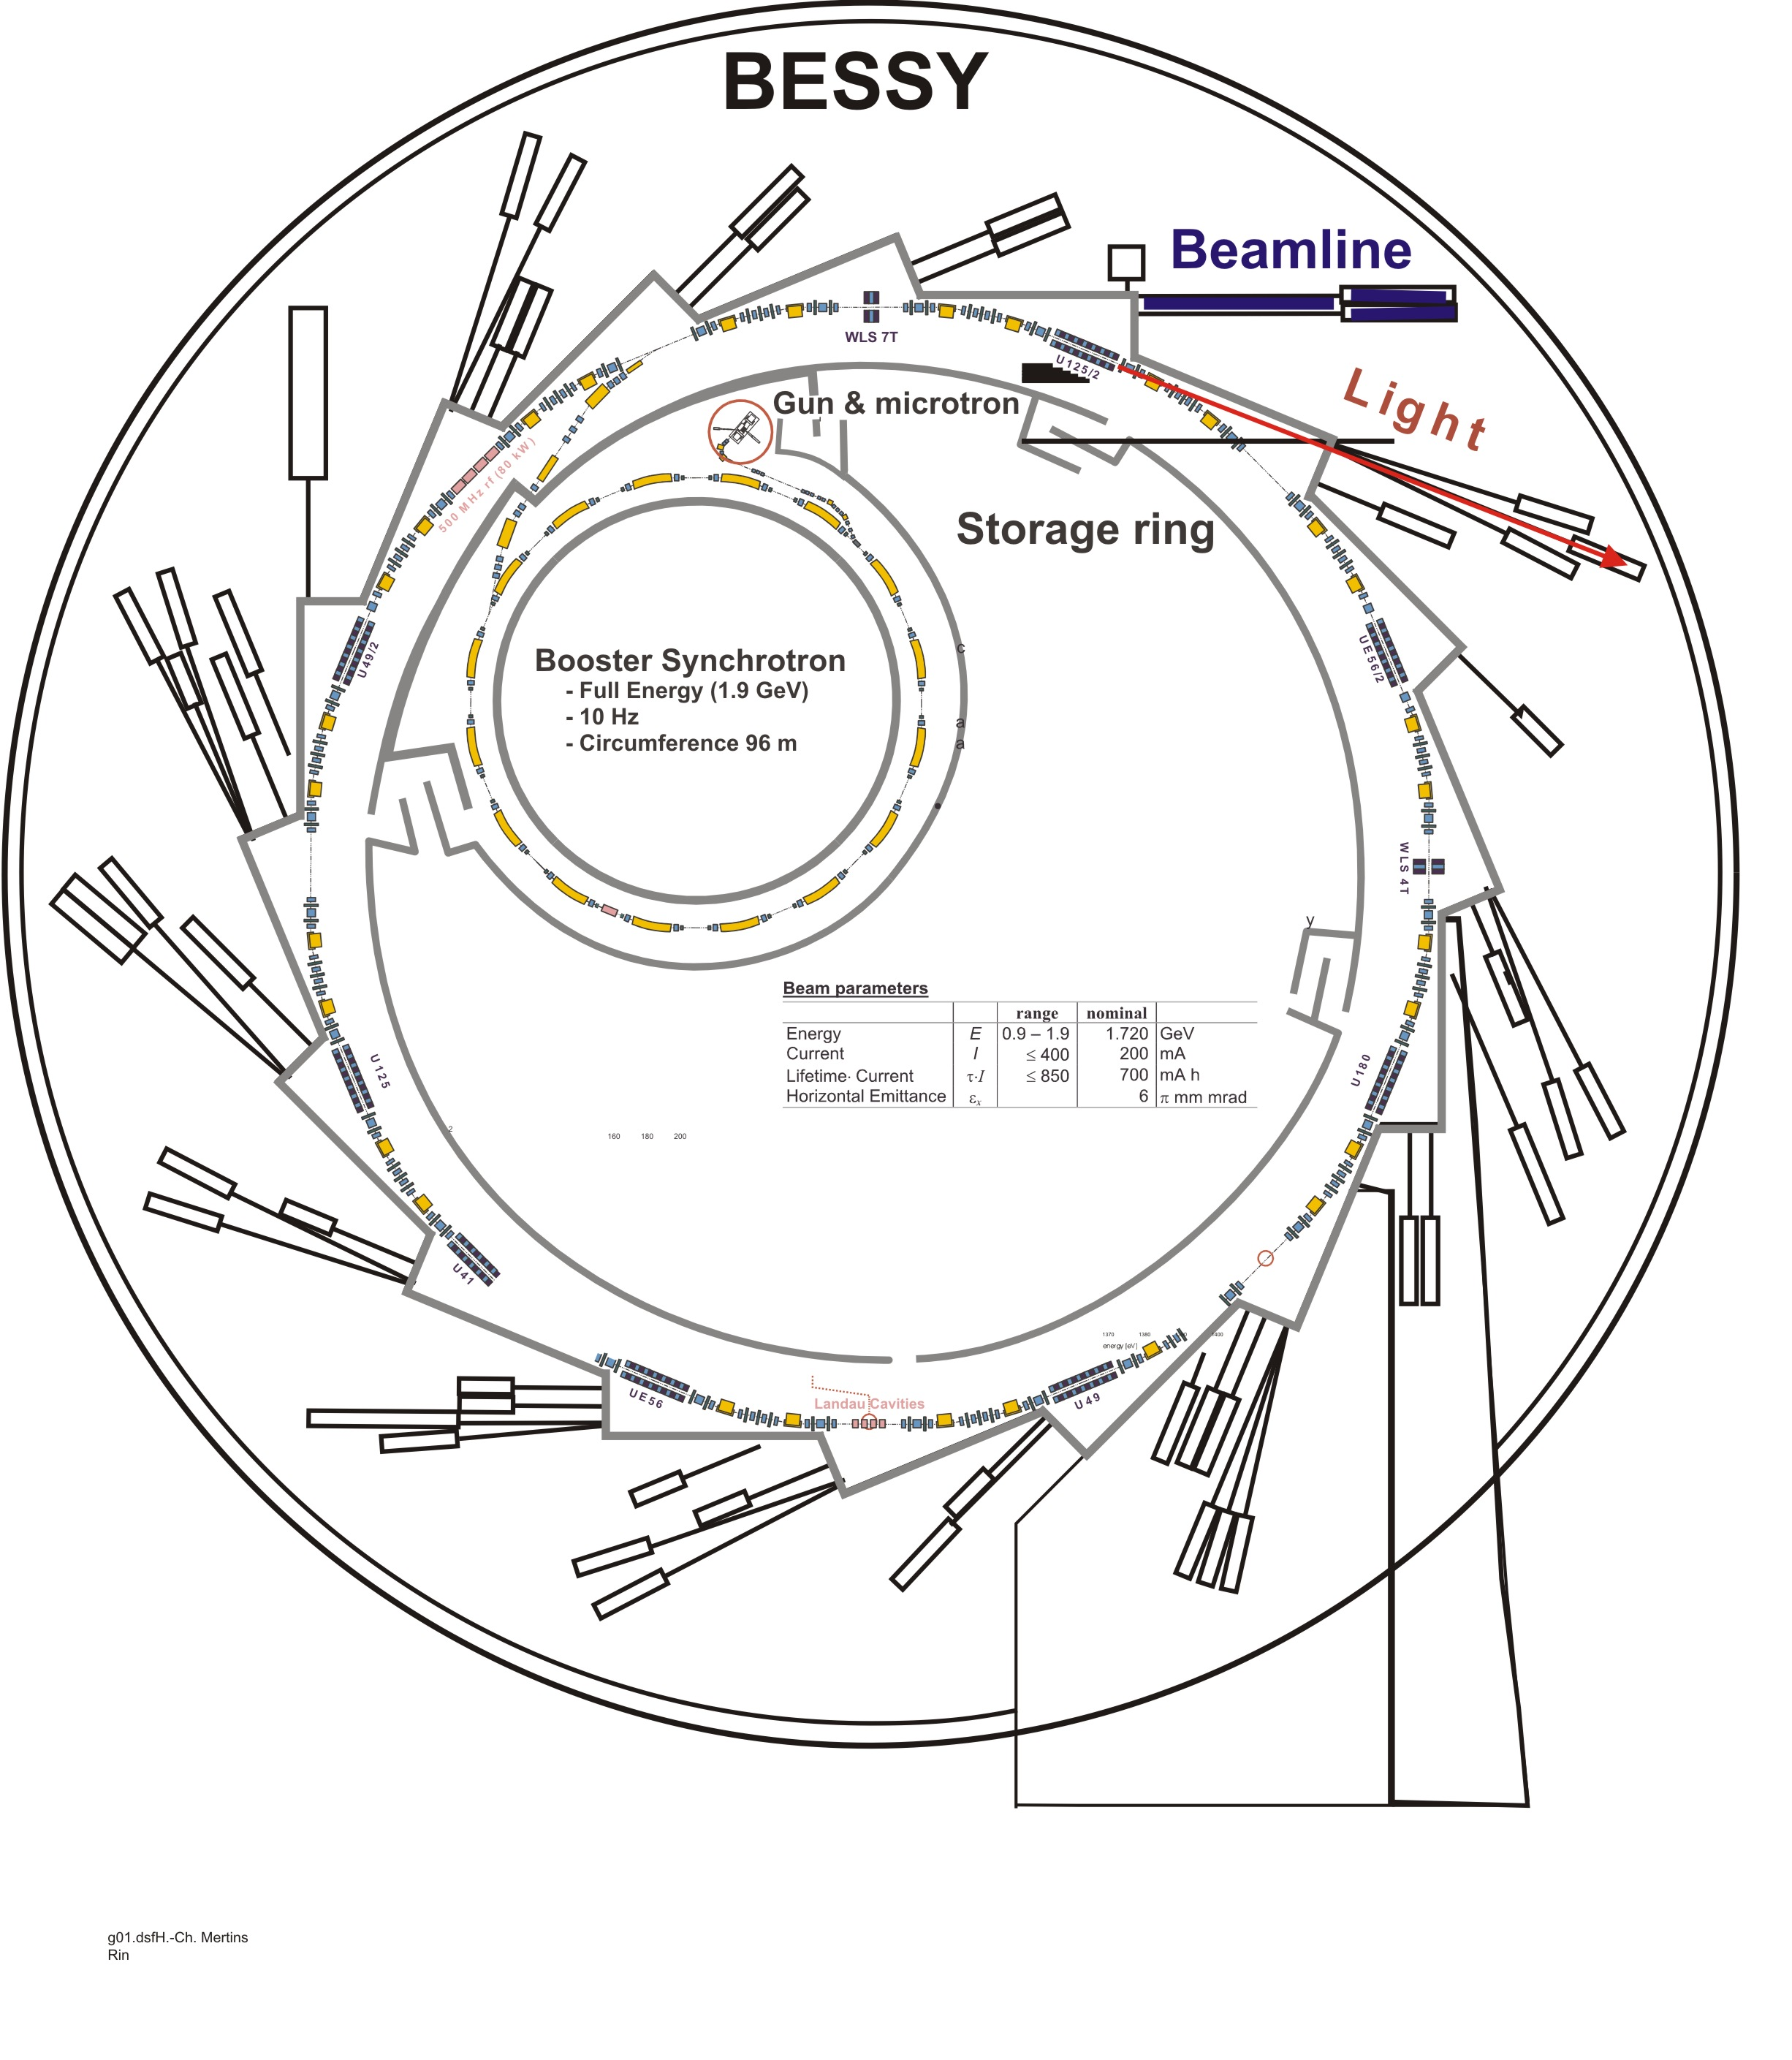
\includegraphics[width=0.8\textwidth]{img/bessy_acc_chain_web.jpg}
    \caption[BESSY~II -- Accelerator chain]{\label{fig:bessy_acc_web_simple} BESSY~II -- Accelerator chain (Source:~\cite{web:bessy_homepage})}
\end{figure}

\begin{sidewaysfigure}
    \centering
    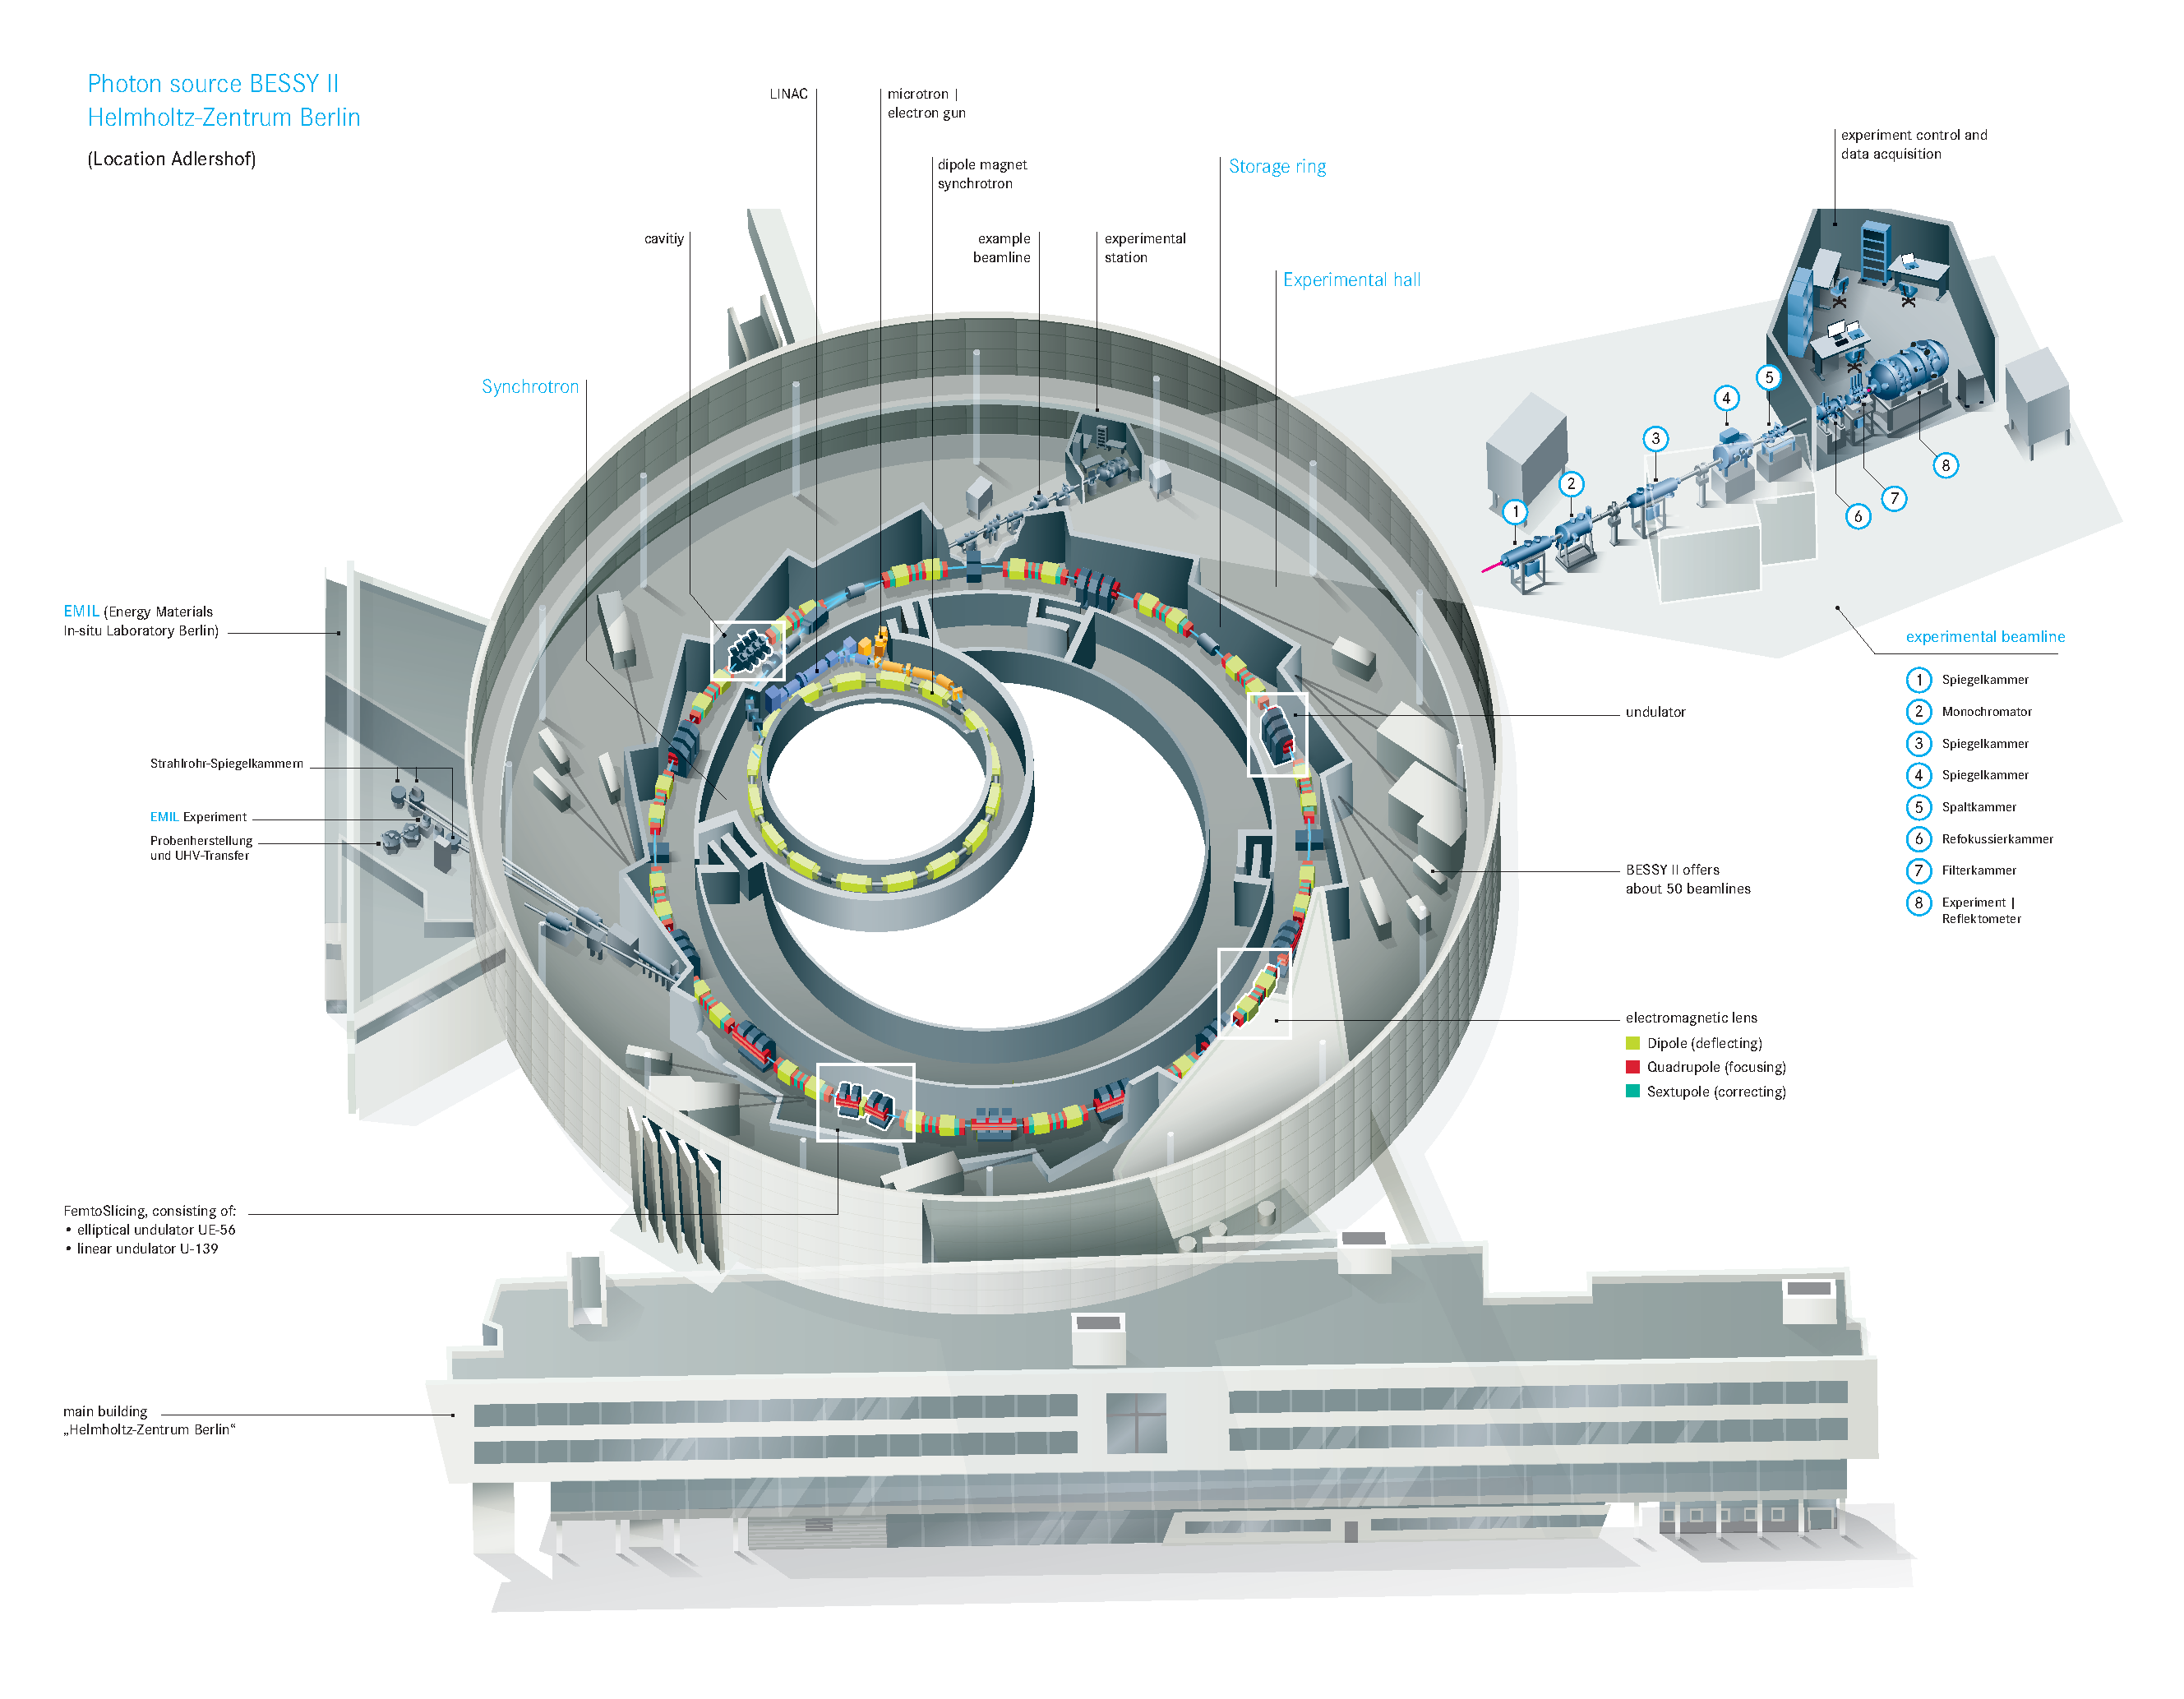
\includegraphics[width=0.8\textwidth,height=0.8\textheight,keepaspectratio]{img/bessy_acc_web.pdf}
    \caption[BESSY~II facility]{\label{fig:bessy_acc_web} BESSY~II facility (Source:~\cite{web:bessy_homepage})}
\end{sidewaysfigure}

In order to reach an energy of \SI{1.7}{\giga\electronvolt}, the electrons undergo several chained accelerations (see \cref{fig:bessy_acc_web}), namely:
\begin{enumerate}
    \item DC eletrons are provided by an electron gun at an energy of \SI{90}{\kilo\electronvolt},
    \item a LINAC (\textbf{lin}ear \textbf{ac}celerator) increase the energy to \SI{50}{\mega\electronvolt},
    \item the booster (a fast rumping synchrotron) accelerate the particles to their full energy of \SI{1.7}{\giga\electronvolt} in not more than \SI{30}{\milli\second}.
\end{enumerate}

When this energy is reached, the electrons are injected to the storage ring, which ensure that the electrons are kept at the same energy.

Another important property of BESSY~II is that it functions in \textit{top-up mode}. This means that its current must be constant over time (in this case: \SI{300}{\milli\ampere}). However electrons are likely to collide into each other or with the rest-gas atoms of the vacuum chamber. To achieve the top-up mode and counter the loss of electrons, new injections from the acceleration chain take place every 2~s to repopulate the storage ring.

\section{Motivation}
The most important properties of the synchrotron radiation are its brilliance and brightness, which represent the quality of the beam. The brightness describes the angular divergence of the beam, and the brilliance includes its transverse dimension: both are expected to be as small as possible to be in the configuration in which the beam is the most point-like. (See \cref{apx:brightness_brilliance} for the exact definitions).

The main purpose of BESSY~II is to provide a light radiation with high brilliance and brightness over time. To achieve this, the light source itself must be very stable and the electron beam very small. The stability of the orbit is required to be well bellow the transverse beam dimensions, which are for BESSY~II storage ring \SI{100}{\micro\meter} in the horizontal direction and \SI{20}{\micro\meter} in the vertical one.

Therefore a significant attention is drawn to the control of the storage ring orbit: the beam diameter must be as small as possible and therefore always well centered in the vacuum chamber. Although the storage ring is designed for to achieve this, perturbations or misalignment in the accelerator optics must be corrected. Orbit feedback is used here to correct and stabilize the orbit and to keep it focused.

\section{Summary}
BESSY~II is a powerful light source, with a nominal energy of \SI{1.7}{\giga\electronvolt}, that produces a light of high quality, which is a wide spectrum and high brilliance. To keep the quality of these properties, orbit correction is needed. This can be achieved by removing perturbation sources and correcting the orbit.

In the following, \cref{sec:acc_physics} will provide the needed accelerator physics backgrounds. \Cref{sec:localization,sec:correction} respectively treat of localization and correction methods.
